\documentclass{article}
\usepackage{pgfplots}
\usetikzlibrary{arrows}
\usetikzlibrary{calc}
\usepackage{amssymb}
\usepackage{amsmath}
\usepackage{subfigure}
\usepackage{siunitx}

\title{ AP Calculus AB Quarter 1 Take-Home Final }
\begin{document}
\author{
	Duncan Freeman
}

\maketitle

\tikzset{
	jumpdot/.style={mark=*,solid},
  excl/.append style={jumpdot,fill=white},
  incl/.append style={jumpdot,fill=black},
}

\section{Fill rate of an inverted cone}
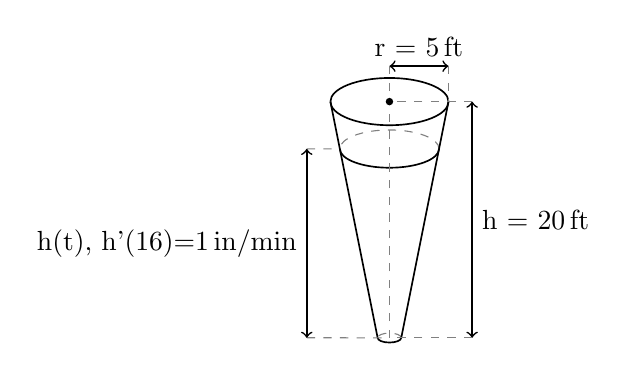
\begin{tikzpicture}[scale=0.15]
	% Cone
	\begin{scope}
		% Cone base
		\coordinate (coneleft) at (-5,0);
		\coordinate (coneright) at (5,0);
		\draw[semithick] (coneright) arc (0:180:5.0 and 2.0);
		\draw[semithick] (coneright) arc (0:180:5.0 and -2.0);

		% Mid cone
		\coordinate (conebottomleft) at (-1.0, -20);
		\coordinate (conebottomright) at (1.0, -20);
		\draw[semithick] (conebottomright) arc (0:180:1.0 and -0.4);
		\draw[dashed, color=gray] (conebottomright) arc (0:180:1.0 and 0.4);

		% Mid line
		\coordinate (conemidleft) at ($(conebottomleft)!0.8!(coneleft)$);
		\coordinate (conemidright) at ($(conebottomright)!0.8!(coneright)$);
		\draw[semithick] (conemidright) arc (0:180:4.2 and -1.6);
		\draw[dashed, color=gray] (conemidright) arc (0:180:4.2 and 1.6);

		% Lines to top
		\coordinate (top) at (0.0, -20.0);
		\draw[semithick] (coneleft) -- (conebottomleft);
		\draw[semithick] (coneright) -- (conebottomright);

		% Side line arrows (H)
		\coordinate (harrowtop) at (7,-20);
		\coordinate (harrowbottom) at (7,0);
		\draw[semithick, <->] (harrowbottom)--(harrowtop) node [midway, right] { h = 20\thinspace ft };
		\draw[dashed, color=gray] (harrowbottom)--(0,0);
		\draw[dashed, color=gray] (harrowtop)--(top);

		% Side line arrows (M)
		\path let \p1 = (conemidleft) in coordinate (arrowmidleft) at (-7,\y1);
		\path let \p1 = (top) in coordinate (arrowbottomleft) at (-7,\y1);
		\draw[dashed, color=gray] (arrowmidleft)--(conemidleft);
		\draw[dashed, color=gray] (arrowbottomleft)--(top);
		\draw[semithick,<->] (arrowbottomleft)--(arrowmidleft) node [midway, left] { h(t), h'(16)=1\thinspace in/min };

		% Side line arrows (R)
		\coordinate (rarrowright) at (5, 3);
		\coordinate (rarrowleft) at (0,3);
		\draw[semithick, <->] (rarrowleft)--(rarrowright) node [midway, above] { r = 5\thinspace ft };
		\draw[dashed, color=gray] (rarrowleft)--(0,0);
		\draw[dashed, color=gray] (rarrowright)--(coneright);

		\draw[dashed, color=gray] (top)--(0,0);
		\fill (0,0) circle[radius=9pt];
	\end{scope}

\end{tikzpicture}

We can relate the height of the cone $h$ and the radius of the cone $r$ by the following...:
\begin{eqnarray}
	\frac{r}{h} = \frac{5}{20} \\
	r = \frac{5}{20}h
\end{eqnarray}

...So that we can find the volume of the cone based on the height function $h(t)$:
\begin{eqnarray}
	V = \frac{\pi r^2 h(t)}{3}
	 = \frac{\pi (\frac{5h(t)}{20})^2 h(t)}{3}
	 = \frac{\pi (\frac{h(t)}{4})^2 h(t)}{3} 
	 = \frac{\pi \frac{h(t)^2}{16} h(t)}{3}
	 = \frac{\pi h(t)^3}{3 * 16}
	 = \frac{\pi h(t)^3}{48}
\end{eqnarray}

Because we want to know the rate of actual increase in volume of the cone $\frac{\Delta V}{\Delta t}$, we need to take the derivate of the above function, then plug the original values in:
\begin{eqnarray}
	\frac{\Delta V}{\Delta t} 
	= \frac{3 \pi h^2 h'}{48} 
	= \frac{\pi h^2 h'}{16}
	= \frac{\pi (16)^2 \frac{1}{12}}{16}
	= \frac{\pi (16)^2}{16 * 12}
	= \frac{16\pi}{12}
	= \frac{4\pi}{3} ft^3/min
\end{eqnarray}

We can then find the rate of the leak by subtracting the calulated rate from the infill rate like so:
\begin {equation}
	8 - \frac{4\pi}{3} \approx 3.811 ft^3/min
\end {equation}

\section{Dimensions of a cylinder}

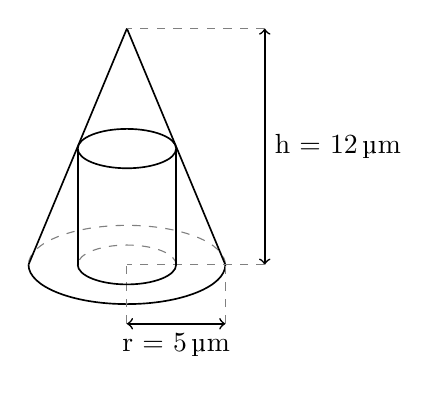
\begin{tikzpicture}[scale=0.25]
	% Cone
	\begin{scope}
		% Cone base
		\coordinate (coneleft) at (-5,0);
		\coordinate (coneright) at (5,0);
		\draw[dashed,color=gray] (coneright) arc (0:180:5.0 and 2.0);
		\draw[semithick] (coneright) arc (0:180:5.0 and -2.0);

		% Lines to top
		\coordinate (top) at (0.0, 12.0);
		\draw[semithick] (coneleft) -- (top);
		\draw[semithick] (coneright) -- (top);

		\coordinate (harrowtop) at (7,12);
		\coordinate (harrowbottom) at (7,0);
		\draw[semithick, <->] (harrowbottom)--(harrowtop) node [midway, right] (htext) { h = \SI{12}{\micro\metre} };
		\draw[dashed, color=gray] (harrowbottom)--(0,0);
		\draw[dashed, color=gray] (harrowtop)--(top);

		\coordinate (rarrowright) at (5, -3);
		\coordinate (rarrowleft) at (0,-3);
		\draw[semithick, <->] (rarrowleft)--(rarrowright) node [midway, below] (rtext) { r = \SI{5}{\micro\metre} };
		\draw[dashed, color=gray] (rarrowleft)--(0,0);
		\draw[dashed, color=gray] (rarrowright)--(coneright);
	\end{scope}

	% Cylinder
	\begin{scope}
		\coordinate (cylleftbottom) at (-2.5,0);
		\coordinate (cylrightbottom) at (2.5,0);
		\draw[dashed,color=gray] (cylrightbottom) arc (0:180:2.5 and 1.0);
		\draw[semithick] (cylrightbottom) arc (0:180:2.5 and -1.0);

		\coordinate (cyllefttop) at (-2.5,5.9);
		\coordinate (cylrighttop) at (2.5,5.9);
		\draw[semithick] (cylrighttop) arc (0:180:2.5 and 1.0);
		\draw[semithick] (cylrighttop) arc (0:180:2.5 and -1.0);

		\draw[semithick] (cyllefttop)--(cylleftbottom);
		\draw[semithick] (cylrighttop)--(cylrightbottom);
	\end{scope}
\end{tikzpicture}

Relationship between $h$ and $r$:
\begin{eqnarray}
	\frac{h}{r} = \frac{12}{5} \\
	h = 12 - \frac{12}{5}r
\end{eqnarray}
Note that as $r$ increases, $h$ must decrease so we subtract the related $h$ from height of the cylinder
\newline
\newline
Volume of the cylinder:
\begin{eqnarray}
	V = \pi r^2 h \\
	V = \pi r^2 \left( 12 - \frac{12}{5}r \right) \\
	V = 12 \pi r^2 - \frac{12 \pi r^3}{5}
\end{eqnarray}

Because this is an optimization problem, we want to find the zeroes of the derivative in order to determine the absolute maximum of the volume.
\begin{eqnarray}
	\frac{\Delta V}{\Delta r} = 24 \pi r - \frac{36 \pi r^2}{5} = 0 \\
	24 \pi r = \frac{36 \pi r^2}{5} \\
	2 = \frac{3 r}{5} \\
	10 = 3r \\
	r = \frac{10}{3} \approx \SI{3.3}{\micro\metre}
\end{eqnarray}

We can then find h from our original relation:
\begin{eqnarray}
	h = 12 - \frac{12}{5} \frac{10}{3} = \SI{4.0}{\micro\metre}
\end{eqnarray}

\section{Curve Sketching}
First, we have to find the first and second derivatives of the function:
\begin{eqnarray}
	y = \frac{e^x}{x-1} \\
	y' = \frac{e^x (x-1) - e^x * 1}{(x-1)^2} 
	= \frac{e^x (x-2)}{(x-1)^2} \\
	y'' = \frac{e^x (x-1) * (x-1)^2 - e^x (x-2) * 2 * (x-1)}{(x-1)^4} 
	= \frac{e^x (x-1)^2 - e^x (x-2) * 2 }{(x-1)^3} \\
	= \frac{e^x \left[(x-1)^2 -(x-2) * 2\right] }{(x-1)^3}
	= \frac{e^x \left(x^2 -2x + 1 -2x + 4\right) }{(x-1)^3}
	= \frac{e^x \left(x^2 -4x + 5\right) }{(x-1)^3}
\end{eqnarray}

We can extract $2$ as a critical number from $(x-2)$ in the first derivative, and $1$ from $(x-1)^3$. $f(1)$ is undefined, however. 
\newline
Now what we have the function, and its first and second derivatives, we can start finding out the behaviour of the function at it's critical points.  
\newline
\newline
\begin{tabular}{ r | c c l l }
	range & $y'$ & $y''$ & behaviour & concavity \\
	\hline
	($-\infty$, 1) & - & - & decreasing & concave down \\
	(1, 2)         & - & + & decreasing & concave up \\
	(2, $\infty$)  & + & + & increasing & concave up \\
\end{tabular}

\begin{eqnarray}
	\lim_{x \to 1^-} \frac{e^x}{x-1} = \frac{e}{0^-} = -\infty \\
	\lim_{x \to 1^+} \frac{e^x}{x-1} = \frac{e}{0^+} = +\infty
\end{eqnarray}

NOTE: SEE ATTACHED MANUAL SKETCH OF THE GRAPH

\section{Definition of a derivative}
\begin{eqnarray}
	y = \frac{5}{\sqrt{2x+1}} \\
	y' = m = \lim_{h \to 0} \frac{\frac{5}{\sqrt{2(h+a)+1}} - \frac{5}{\sqrt{2a+1}}}{h}
	= \frac{\frac{5}{\sqrt{2(h+4)+1}} - \frac{5}{\sqrt{2(4)+1}}}{h}
	= \frac{\frac{5}{\sqrt{2h+9}} - \frac{5}{\sqrt{9}}}{h} \\
	= \frac{\frac{5}{\sqrt{2h+9}} - \frac{5}{\sqrt{9}}}{h} * \frac{\sqrt{9}\sqrt{2h+9}}{\sqrt{9}\sqrt{2h+9}}
	= \frac{5(3) - 5\sqrt{2h + 9}}{3h\sqrt{2h+9}} \\
	= \frac{15 - 5\sqrt{2h + 9}}{3h\sqrt{2h+9}} 
	* \frac{15 + 5\sqrt{2h + 9}}{15 + 5\sqrt{2h + 9}} 
	= \frac{255-25(9 + 2h)}{h(3\sqrt{9+2h})(15 + 5\sqrt{9+2h})} \\
	= \frac{255-255 - 50h)}{h(3\sqrt{9+2h})(15 + 5\sqrt{9+2h})}
	= \frac{-50}{(3\sqrt{9+2h})(15 + 5\sqrt{9+2h})} \\
	lim_{h \to 0} \frac{50}{(3\sqrt{9+2h})(15 + 5\sqrt{9+2h})}  
	= \frac{-50}{(3\sqrt{9})(15 + 5\sqrt{9})}
	= \frac{-50}{9 * (15 + 5(3))} = \frac{-50}{270} = \frac{-5}{27}
\end{eqnarray}

And now that we know $m$ we can get the line equation:
\begin{equation}
	y - \frac{5}{3} = \frac{-5}{27} (x - 4)
\end{equation}

\section{Particle Movement}
First, we write out and derive the particle motion:
\begin{eqnarray}
	f(t) = 40t^3 - 333t^2 + 810t + 20 \text{ where } 0 \leq t \leq 7 \\
	f'(t) = 120t^2 - 666t + 810 \\
	f''(t) = 120t - 666
\end{eqnarray}

Next, we find the critical numbers by finding the zeroes of $f'(t)$ and $f''(t)$:
\begin{eqnarray}
	0 = f'(t) = 120t^2 - 666t + 810 \\
	t = \frac{666}{2 * 120} \pm \frac{\sqrt{666^2 - 4(120)(810)}}{2 * 120}
	= \frac{333}{120} \pm \frac{117}{120} \approx 1.8, 3.75 
\end{eqnarray}

\begin{tabular}{ r | c c c l }
	range & $y'$ & $y''$ & direction & action \\
	\hline
	(0, 1.8)    & + & - & forward & slowing down \\
	(1.8, 3.75) & - & - & backward & slowing down \\
	(3.75, 7)   & + & + & forward & speeding up \\
\end{tabular}

We can now find the total distance travelled by computing:
\begin {equation}
	|k(0) - k(1.8)| + |k(1.8) - k(3.75)| + |k(3.75) - k(7)| = 3369.595 m
\end {equation}

\begin{tikzpicture}[]
	\begin{axis}[
			xmin=-0.1,xmax=7,
		  ymin=20,ymax=2900,
		  axis x line=middle,
		  axis y line=left,
		  xlabel={$x$},
		  ylabel={$y$},
		]
		  \addplot[blue,<->] expression[domain=0:7,samples=100]{40*(x^3) - 333*(x^2) + 810*x + 20};
		  \addplot[incl,blue] coordinates {(-5,5)};
	\end{axis}
\end{tikzpicture}

\section{Wire Length}
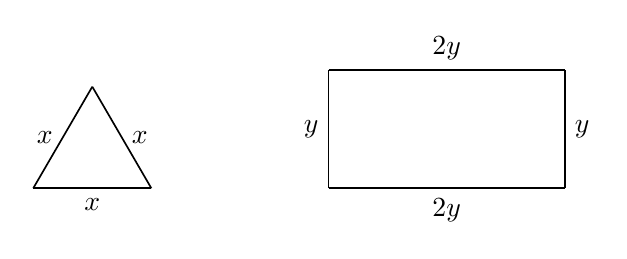
\begin{tikzpicture}[scale = 1.5]
	\coordinate (a) at (0, 0.86);
	\coordinate (b) at (-0.5, 0);
	\coordinate (c) at (0.5, 0);
	\draw[semithick] (a)--(c) node [midway, right] {$x$};
	\draw[semithick] (a)--(b) node [midway, left] {$x$};
	\draw[semithick] (b)--(c) node [midway, below] {$x$};

	\draw[semithick] (2,0) -- (2, 1) node [midway, left] {$y$};
	\draw[semithick] (2,1) -- (4, 1) node [midway, above] {$2y$};
	\draw[semithick] (4,1) -- (4, 0) node [midway, right] {$y$};
	\draw[semithick] (2,0) -- (4, 0) node [midway, below] {$2y$};
\end{tikzpicture}

The wire length relation is so:
\begin{eqnarray}
	15 = 6y + 3x \\
	y = \frac{15 - 3x}{6}
\end{eqnarray}

The combined area of the shapes is:
\begin{equation}
	\frac{x^2 \sqrt{3}}{4} + y * 2y 
	= \frac{x^2 \sqrt{3}}{4} + 2y^2 
	= \frac{x^2 \sqrt{3}}{4} + 2\left(\frac{15 - 3x}{6}\right)^2 
\end{equation}

To maximize the area of both shapes, we need to take the derivative of the area function, like so:
\begin{eqnarray}
	A' = \frac{4*2x\sqrt{3} - 0*x^2\sqrt{3}}{4^2} + 2 * 2 * \left(\frac{15-3x}{6}\right) * \frac{-3x}{6}
	= \frac{8x\sqrt{3}}{16} - 12x\left(\frac{15-3x}{6}\right) \\
	= \frac{8x\sqrt{3}}{16} - \frac{36x^2 - 180x}{6}
	= \frac{1}{2}\sqrt{3}x + 6x^2 - 30x
	= 6x^2 + x\left(\frac{1}{2}\sqrt{3} - 30\right) = 0 \\
	x = \frac{-b}{2a} = \frac{-\frac{1}{2}\sqrt{3} + 30}{2 * 6} \approx 2.4278
\end{eqnarray}

Which means we cut at about $2.4278$ meters after the beginning of the wire. 

\section{Ladder and related rates}
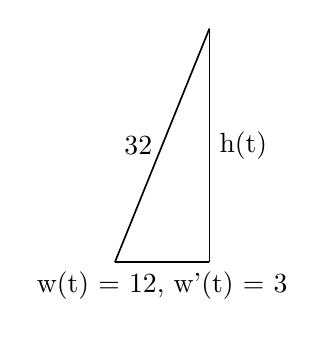
\begin{tikzpicture}[scale = 0.1]
	\coordinate (a) at (0,0);
	\coordinate (b) at (12, 29.664);
	\coordinate (c) at (12,0);
	\draw[semithick] (a) -- (b) node [midway, left] {32};
	\draw[semithick] (a) -- (c) node [midway, below] {w(t) = 12, w'(t) = 3};
	\draw[semithick] (b) -- (c) node [midway, right] {h(t)};
\end{tikzpicture}

The height and width of the triangle can be related by pythagorean theorem: 
\begin{eqnarray}
	32 = \sqrt{h(t)^2 + w(t)^2} \\
	32^2 = h(t)^2 + w(t)^2 \\
	\sqrt{32^2 - w(t)^2} = h(t)
\end{eqnarray}

Now, height can be defined as a function of time:
\begin{eqnarray}
	\frac{\Delta h}{\Delta t} h(t) = \frac{w'(t)}{\sqrt{32^2 - w(t)^2}}
	= \frac{3}{\sqrt{32^2 - (12)^2}} \approx .101 ft/sec
\end{eqnarray}

\section{Graphing a function}
\begin{equation}
	f(x) = 
	\begin{cases} 
		5 & x \leq -5 \\
		2x + 1 & -4 < x < -2 \\ 
		-\sqrt{4-x^2} & -2 < x \leq 2 \\
		x^2 - 4 & 2 < x
	\end{cases}
\end{equation}

\begin{tikzpicture}[]
	\begin{axis}[
			xmin=-7,xmax=3,
		  ymin=-10,ymax=7,
		  axis x line=middle,
		  axis y line=left,
		  xlabel={$x$},
		  ylabel={$y$},
		]
		  \addplot[no marks,blue,<-] expression[domain=-7:-5,samples=10]{5};
		  \addplot[incl,blue] coordinates {(-5,5)};

		  \addplot[no marks,red,-] expression[domain=-5:-2,samples=10]{2*x + 1};
		  \addplot[excl, red, fill=white] coordinates {(-5,-9)};
		  \addplot[excl, red, fill=white] coordinates {(-2,-3)};

		  \addplot[no marks,green,-] expression[domain=-2:2,samples=100]{-sqrt(4-(x^2))};
		  \addplot[excl, green, fill=white] coordinates {(-2,0)};

		  \addplot[no marks,magenta,-] expression[domain=2:4,samples=100]{(x^2)-4};
		  \addplot[incl, green, fill=magenta] coordinates {(2,0)};

	\end{axis}
\end{tikzpicture}

The function is non-differentiable at $x=-2$ and continuous at $(-\infty, -2) \cup (-2, \infty)$ 

\end{document}
